\chapter{Encapsulation and Data Hiding}

\section{Introduction: Real-Life Hook}

Think about your school bag.

Inside it you keep:
\begin{itemize}
    \item Books
    \item Exam papers
    \item Personal notes
\end{itemize}

You do not allow everyone to touch or change these things.
You control:
\begin{itemize}
    \item Who can open the bag
    \item What can be taken out
\end{itemize}

In programming, we do the same thing with data.
This idea is called \textbf{Encapsulation}.

\section{Concept: What Is Encapsulation?}

\begin{definition}{Encapsulation}
Encapsulation is an OOP concept where \textbf{data and methods are kept together}, and direct access to data is restricted.
\end{definition}

Encapsulation means:
\begin{itemize}
    \item Wrapping data and methods into one unit (class)
    \item Protecting data from unwanted access
\end{itemize}

\section{Why Encapsulation Is Needed}

Without encapsulation:
\begin{itemize}
    \item Anyone can change data wrongly
    \item Bugs increase
    \item Programs become unsafe
\end{itemize}

With encapsulation:
\begin{itemize}
    \item Data is protected
    \item Code is clean
    \item Programs are reliable
\end{itemize}

\section{Real-Life Example}

A bank account:
\begin{itemize}
    \item Balance is private
    \item You cannot change balance directly
    \item You must use deposit or withdraw
\end{itemize}

This is exactly how encapsulation works.

\section{Encapsulation in Python}

Python uses naming rules to protect data.

\subsection{Public Members}

Accessible everywhere.

\begin{verbatim}
class Student:
    def __init__(self, name):
        self.name = name
\end{verbatim}

\subsection{Private Members}

Use double underscore \texttt{\_\_}

\begin{verbatim}
class BankAccount:
    def __init__(self, balance):
        self.__balance = balance
\end{verbatim}

\section{Accessing Private Data Using Methods}

\begin{verbatim}
class BankAccount:
    def __init__(self, balance):
        self.__balance = balance

    def deposit(self, amount):
        self.__balance += amount

    def get_balance(self):
        return self.__balance
\end{verbatim}

\begin{verbatim}
acc = BankAccount(1000)
acc.deposit(500)
print(acc.get_balance())
\end{verbatim}

\textbf{Output:}
\begin{verbatim}
1500
\end{verbatim}

\section{Data Hiding}

\begin{definition}{Data Hiding}
Data hiding means \textbf{keeping internal data hidden and allowing access only through methods}.
\end{definition}

It prevents:
\begin{itemize}
    \item Accidental changes
    \item Security issues
    \item Logical errors
\end{itemize}

\section{Getter and Setter Methods}

\subsection{Getter}

Used to read data.

\begin{verbatim}
def get_balance(self):
    return self.__balance
\end{verbatim}

\subsection{Setter}

Used to modify data safely.

\begin{verbatim}
def set_balance(self, amount):
    if amount >= 0:
        self.__balance = amount
\end{verbatim}

\section{Mini-Project: Student Result System}

\textbf{Goal:} Protect student marks.

\begin{verbatim}
class Student:
    def __init__(self, name, marks):
        self.name = name
        self.__marks = marks

    def get_marks(self):
        return self.__marks

    def set_marks(self, new_marks):
        if 0 <= new_marks <= 100:
            self.__marks = new_marks
        else:
            print("Invalid marks")
\end{verbatim}

\begin{verbatim}
s = Student("Rahim", 80)
s.set_marks(90)
print(s.get_marks())
\end{verbatim}

Students learn:
\begin{itemize}
    \item Safe data handling
    \item Real-life validation
    \item Encapsulation benefits
\end{itemize}

\section{Diagram: Encapsulation Model}

\begin{center}
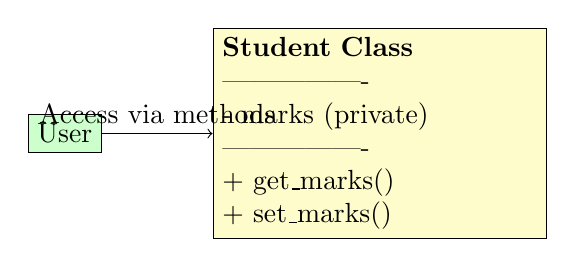
\begin{tikzpicture}[node distance=4cm]
\node (class) [draw, rectangle, fill=yellow!20, text width=4cm, align=left] {
\textbf{Student Class}\\
----------------\\
- marks (private)\\
----------------\\
+ get\_marks()\\
+ set\_marks()
};

\node (user) [draw, rectangle, fill=green!20, left of=class] {User};

\draw[->] (user) -- node[above] {Access via methods} (class);
\end{tikzpicture}
\end{center}

\section{Advantages of Encapsulation}

\begin{itemize}
    \item Improves security
    \item Controls data access
    \item Makes code easy to maintain
    \item Supports modular programming
\end{itemize}

\section{Key Concepts}

\begin{itemize}
    \item Encapsulation bundles data and methods
    \item Private variables protect data
    \item Getters and setters control access
    \item Data hiding improves program safety
\end{itemize}

\section{Common Beginner Mistakes}

\begin{itemize}
    \item Accessing private variables directly
    \item Not using validation in setters
    \item Making all data public
\end{itemize}

\section{End-of-Chapter Exercises}

\subsection{Very Short Questions}

\begin{enumerate}
    \item What is encapsulation?
    \item What symbol makes a variable private in Python?
    \item What is data hiding?
\end{enumerate}

\subsection{Short Answer Questions}

\begin{enumerate}
    \item Explain encapsulation using a real-life example.
    \item Why are getter and setter methods important?
    \item What problems occur without encapsulation?
\end{enumerate}

\subsection{Activity-Based Exercises}

\begin{enumerate}
    \item Create a \texttt{MobilePhone} class with private IMEI number.
    \item Design a \texttt{LibraryBook} class with protected availability status.
    \item Modify a program to add data validation using setters.
\end{enumerate}

\section{Teacher Notes}

\marginnote{
\textbf{Learning Objectives}
\begin{itemize}
    \item Students understand encapsulation clearly
    \item Students use private variables correctly
    \item Students apply data hiding
\end{itemize}

\textbf{Teaching Tips}
\begin{itemize}
    \item Use school bag or locker analogy
    \item Show wrong access problems
    \item Emphasize safety of data
\end{itemize}

\textbf{Assessment}
\begin{itemize}
    \item Proper encapsulation usage
    \item Getter-setter correctness
\end{itemize}
}